\documentclass[times, utf8, zavrsni, numeric]{fer}
\usepackage{booktabs}
\usepackage{graphicx}
\usepackage{amsmath}
\usepackage{courier} %% Sets font for listing as Courier.
\usepackage{listings, xcolor}
\lstset{
	tabsize = 4, %% set tab space width
	showstringspaces = false, %% prevent space marking in strings, string is defined as the text that is generally printed directly to the console
	numbers = left, %% display line numbers on the left
	commentstyle = \color{green}, %% set comment color
	keywordstyle = \color{blue}, %% set keyword color
	stringstyle = \color{red}, %% set string color
	rulecolor = \color{black}, %% set frame color to avoid being affected by text color
	basicstyle = \small \ttfamily , %% set listing font and size
	breaklines = true, %% enable line breaking
	numberstyle = \tiny,
}
\begin{document}

% TODO: Navedite broj rada.
\thesisnumber{6623}

% TODO: Navedite naslov rada.
\title{Primjena bojanja vrhova grafa u izradi rasporeda ispita}

% TODO: Navedite vaše ime i prezime.
\author{Antonio Filipović\\
Voditelj: izv. prof. dr. sc. Tomislav Burić}

\maketitle



% Dodavanje zahvale ili prazne stranice. Ako ne želite dodati zahvalu, naredbu ostavite radi prazne stranice.
\zahvala{Zahvaljujem svojoj majci i ocu što su me oduvijek podržavali.}

\tableofcontents

\chapter{Uvod}
U razdoblju velike računalne snage, mnogi zadatci koje bi ljudi morali sami rješavati pokušavaju se automatizirati i kako bi život čovjeku  bio jednostavniji. No, iako mnogi gledaju na računala kao stroj koji će sam od sebe riješti sve naše probleme, ona su ipak samo alat. Ono što je istina je da iza svih tih automatiziranih procesa stoji čovjek koji koristeći se računalom kao alatom traži rješenja svojih problema. Jedan od takvih problema je i problem slaganja rasporeda ispita tako da ne postoje preklapanja.\par
U rješavanju problema, matematika nam općenito nudi velike mogućnosti. U ovom slučaju okrećemo se k teoriji grafova. Teorija grafova, grana je matematike koja se bavi istraživanjem problema opisanih s pomoću mrežnih grafova. Nazivlje u teoriji grafova razlikuje se od uobičajenoga matematičkog nazivlja: graf je matematički objekt koji se sastoji od skupa vrhova (točaka) i skupa bridova (dužina koje povezuju vrhove).\par 
Problem bojanja grafova jedan je od najpoznatijih problema u području teorije grafova s dugom i slavnom poviješću. Pitanje mogu li se sve zemlje svijeta obojati samo sa 4 boje, tako da one susjedne nisu obojane istom bojom, jedan je od najpoznaijih primjera bojanja grafa.\par
Postoji više načina bojanja grafa. Mogu se bojati vrhovi ili bridovi. U nastavku rada bojanje grafa odnosi se na bojanje vrhova grafa. U suštini, problem se svodi na pridruživanje boje svakom vrhu tako da su zadovoljena dva uvjeta. Prvi uvjet traži da niti jedna dva vrha spojena bridom nemaju istu boju. Taj uvjet prilično je lagano zadovoljiti s obzirom da boja u ovom svijetu ima prilično mnogo. Drugi uvjet koji zapravo ograničava prvi je to da broj boja koje pritom koristimo bude minimalan.\par
Ako predmete gledamo kao vrhove, a bridove između njih kao postojanje studenta koji ima ispit iz oba predmete, možemo uočiti da problem izrade rasporeda možemo svesti na bojanje grafova. Općenito se u primjeni pritom uvode i dodatni uvjeti. Iako se na prvi pogled problem ne čini kompliciranim, može se podosta zakomplicirati jer postoje fizička ograničenja. U problemu izrade rasporeda, jedno takvo fizičko ograničenje  maksimalni je kapacitet dvorana u koje se studenti mogu rasporediti. Tu je i uvjet da određeni ispit mora biti u točno određeno vrijeme ili prije nekog drugog ispita. \par
Cilj rada je dakle, primjenom bojanja vrhova grafa, pronaći koliki je minimalan broj termina potreban kako bi se predmeti rasporedili u termine, a da bilo koji student u jednom terminu nema dva ispita, točnije da nema preklapanja u rasporedu. Nadalje, cilj je te termine rasporediti prema danima tako da u pojedinom danu što manji broj studenata ima više od jednog ispita.\par
U radu se daje teorijska podloga grafova, opisuju se vrste grafova i daje se formalna definicija bojanja grafa te se navodi sustav prema kojem je razvijena programska implementacija za raspoeđivanje predmeta po terminima. Također kratko ulazimo i u složenost algoritma bojanja grafa. Dalje se opisuje i programska implementacija, razlike u načinu raspoređivanja termina i navode se objašnjenja korištenih algoritama. Na kraju dana je usporedba korištenih algoritama i dokumentirana je korištena literatura.

\chapter{Teorijski uvod}
 

\section{Teorija grafova}
\label{sec:teorijaGrafova}
Formalno definirano, jednostavni se graf \textit{G} sastoji se od nepraznog konačnog skupa \textit{V(G)}, čije elemente zovemo vrhovi(čvorovi) grafa \textit{G} i konačnog skupa \textit{E(G)} različitih dvočlanih podskupova skupa \textit{E(G)} koje zovemo bridovi. Skup \textit{V(G}) zovemo skup vrhova, a skup \textit{E(G)} zovemo skup bridova. Ponekad ćemo pisati \textit{G = (V(G), E(G))}.

Oznaka za skup vrhova, \textit{V}, dolazi od engleske riječi \textit{vertex} sa značenjem vrh, a oznaka \textit{E} za
skup bridova dolazi pak od engleske riječi \textit{edge} sa značenjem brid.

\begin{figure}[h]
	\centering
	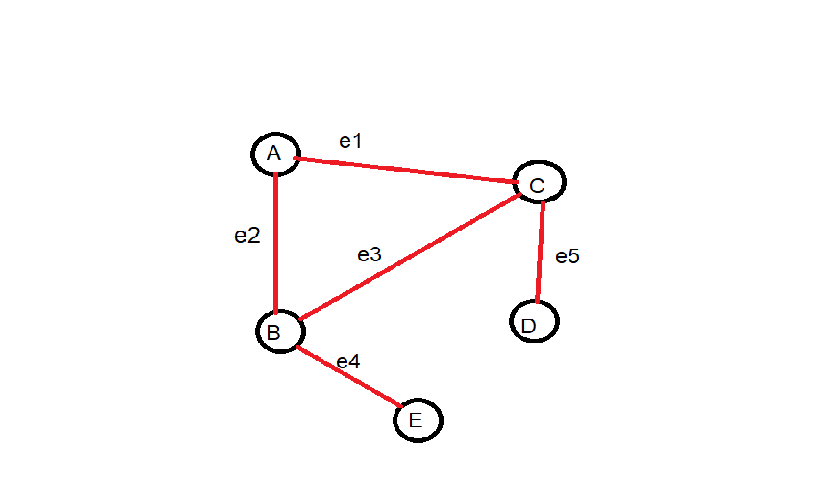
\includegraphics[width=0.8\columnwidth]{slike/graf.png}
	\caption{Jednostavni graf}
	\label{fig:graf}
\end{figure}

Na slici \ref{fig:graf} možemo vidjeti jednostavni graf na kojem su vrhovi su označeni slovima  \textit{A, B, C, D i E}, a bridovi \textit{e1, e2, e3, e4 i e5}.
Bridove jos možemo označavati slovima vrhova koje spajaju.
Tako je u našem slučaju \textit{e1 = AC, e2 = AB, e3 = BC}...


Bridovi grafa mogu biti usmjereni ili neusmjereni. Graf kojemu su svi bridovi usmjereni zovemo usmjerni graf, u suprotnom, zovemo ga neusmjereni. Graf sa slike  \ref{fig:graf} je neusmjeren. U tom primjeru, linija od točke A do točke B identificira se s linijom od točke B do točke A. U usmjerenom grafu (skraćeni naziv digraf), ta dva smjera smatraju se različitim bridovima. Ako graf G nije usmjeren, tada su dva vrha pridružena jednom bridu međusobno ravnopravna. U usmjerenom grafu brid može biti usmjeren od jednog vrha prema drugome. Na slici \ref{fig:usmjereni-neusmjereni}, graf 1 prikazuje primjer neusmjerenog, a graf 2 primjer usmjerenog grafa. 

\begin{figure}[h]
	\centering
	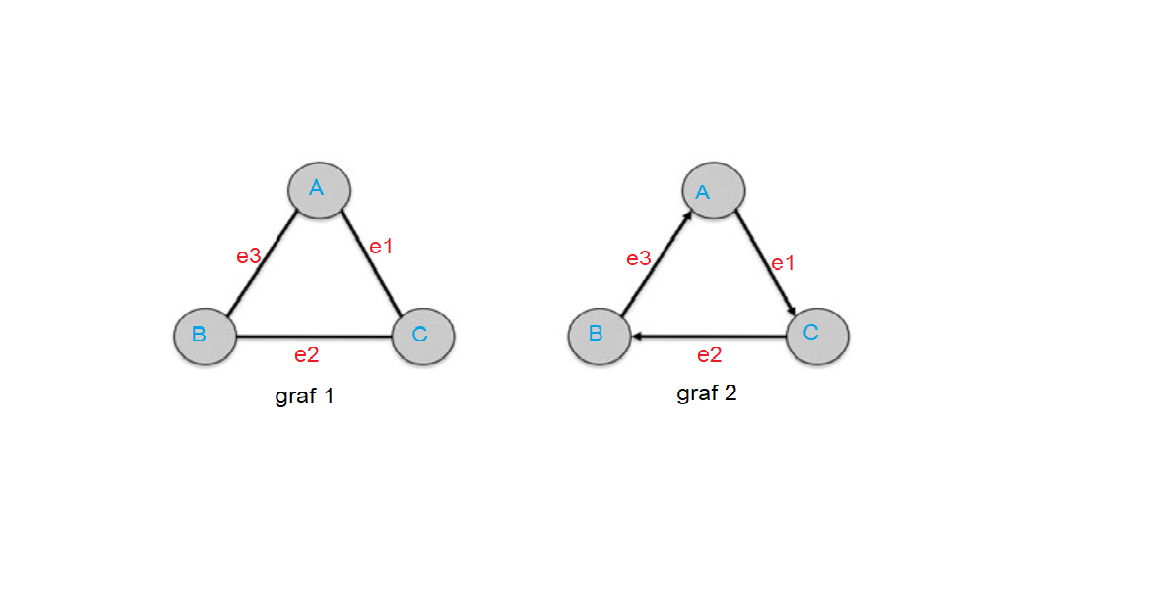
\includegraphics[width=\linewidth]{slike/usmjereni-neusmjereni.png}
	\caption{Usmjereni i neusmjereni graf}
	\label{fig:usmjereni-neusmjereni}
\end{figure}


Grafovi se u računalu mogu reprezentatirati na razne načine. Bitno je jedino da imamo dovoljno podataka kako bi kasnije mogli raditi sa grafovima.

Jedna mogućnost je lista susjedstva. Ona je definirana na način da svakom vrhu pridružimo listu (polje) gdje je elemente liste čini podskup skupa vrhova koji su susjedi dotičnog vrha. Za primjer sa slike \ref{fig:graf} onda vrijedi \textit{[A:(B,C); B:(A,C,E); C:(A,B,D); D:(C); E:()]}
			
Druga mogućnost uključuje označivanje vrhove zadanog grafa \textit{G} sa \textit{V = (1,2,..., n)}. Na tako definiranim vrhovima, definiramo matricu susjedstva \textit{A = [$a_{i,j}$]} kao \textit{n x n} matricu čiji je element $a_{i,j}$ jednak broju bridova koji spajaju vrh \textit{i} s vrhom \textit{j}. Matrica, u matematici, pravokutna je tablica brojeva, ili općenito tablica, koja se sastoji od apstraktnih objekata nad kojima se mogu provoditi računske operacije.
Za primjer sa slike \ref{fig:graf} tada uz preimenovanje vrhova \textit{(A,B,C,D,E)} = \textit{(1,2,3,4,5)} vrijedi:


\begin{equation*}
	A = 
	\begin{bmatrix}
		0 & 1 & 1 & 0 & 0 \\
		1 & 0 & 1 & 0 & 1 \\
		1 & 1 & 0 & 1 & 0 \\
		0 & 0 & 1 & 0 & 0 \\
		0 & 1 & 0 & 0 & 0
		
	\end{bmatrix}
\end{equation*}

Kada razmišljamo o problemu bojanja grafa, treba uzeti u obzir da bridovi nisu usmjereni te grafovi ne mogu sadržavati petlje. Posljedično, matrica A simetrična je ($\textit{$A_{i,j}$}$ = $\textit{$A_{j,i}$}$) i samo sadrži nule po glavnoj dijagonali ($\textit{$A_{i,i}$}$=0). 

Kao što vidimo iz prikazanog, grafovi sa brojem čvorova većim od $10^{5}$ mogu predstavljati probleme u računalnoj implementaciji. U ovom trenutku čak ne toliko u memoriji koliko u pretraživanju susjednih čvorova. Zbog toga teško je reći koji je način bolji. Općenito je rješenje kod takvog problema kombinirati oba načina, jer lista susjedstva bolja je za pretraživanje, a matrica susjedstva za direktno otkrivanje jesu li neka dva čvora susjedna.\par
Dodatno, potrebno je definirati i stupanj vrha grafa. Stupanj vrha \textit{v} grafa G broj je bridova koji su incidentni s vrhom v, što označavamo s \textit{deg(v)}. Ako je vrh \textit{v} petlja, tada ona dogovorno, broju \textit{deg(v)} doprinosi sa 2. Vrh stupnja 0 zovemo izolirani vrh, a vrh stupnja 1 zovemo krajnji vrh. Drugačije rečeno, stupanj je vrha broj sjecišta male kružnice oko vrha sa bridovima koje izlaze iz tog vrha.

\begin{figure}[h]
	\centering
	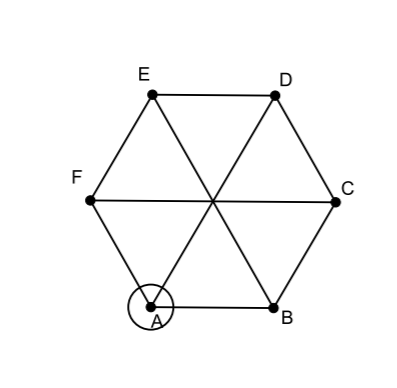
\includegraphics[width=0.5\columnwidth]{slike/stupanj-vrha.png}
	\caption{Stupanj vrha}
	\label{fig:stupanj-vrha}
\end{figure}

Na slici \ref{fig:stupanj-vrha} vidimo da \textit{deg(A})=3 jer kružnicu oko vrha A sijeku 3 brida (prema vrhu F, D te B).\\



\newpage
\section{Bojanje grafova}
U teoriji grafova bojenje grafova se odnosi na specifičan slučaj označavanja grafa odnosno
dodjeljivanje oznaka (boja) elementima grafa uz neka ograničenja.
Bojanje grafa može se provoditi bojanjem vrhova tako da susjedni vrhovi budu različite boje. Drugi slučaj odnosi se na bojanje bridova - uvjet da su dva susjedna brida različite boje.

U nastavku rada kada se govori o bojanju grafa misli se na bojanje vrhova grafa.

Sada treba pružiti formalniju definiciju bojanja grafa. Neka se graf \textit{G = (V,E)} sastoji od \textit{n} vrhova \textit{V} i \textit{m} bridova \textit{E}. U takvom grafu, problem bojanja grafa želi svakom vrhu \textit{v} $\in$  \textit{V}, pridružiti broj \textit{c(v)} $\in$ \textit{(1, 2,..., k)} tako da:
\begin{itemize}
	\item \textit{c(v)}  $\neq$  c(u) $\forall$ \textit{(v,u)} $\in$ E; 
	\item \textit{k} je minimalan.
\end{itemize}.
U ovoj interpretaciji, umjesto stvarnih boja korištenih u početnom primjeru, koristimo oznake \textit{1,2,...,k}. Ako u rješenju se pojavi da je vrhu \textit{v} pridružena boja s oznakom 5, onda to pišemo kao \textit{c(v)} = 5. Prema prvoj točki gore definiranoj, paru vrhova koje spaja brid mora biti pridružena drugačija boja. Druga točka zahtjeva da minimiziramo broj boja koje koristimo.

\vspace{2mm}
Potrebno je sada uvesti određene pojmove.

Za bojanje grafa kaže se da je potpuno ako je svim vrhovima dodijeljena boja \textit{c(v)} $\in$ \textit {(1, . . . , k)}. Inače, bojanje grafa se smatra djelomičnim.

Sukob opisuje situaciju gdje je paru susjednih vrhova \textit{(u, v)} $\in$ \textit{V} dodijeljena ista boja, to jest \textit{{(u, v)}} $\in$ E i \textit{c(v)} = \textit{c(u)}. Ako ne postoji takva situacija, bojanje grafa se smatra pravim, inače nepravim.

Bojanje se smatra izvodljivim ako je i potpuno i pravo.

Kromatski broj u grafu \textit{G}, $\chi$(G), predstavlja minimalni broj boja potreban u izvodljivom bojanju grafa. Izvodljivo bojanje grafa \textit{G} koje koristi točno $\chi$(G) boja smatra se optimalnim.

\begin{figure}[h]
	\centering
	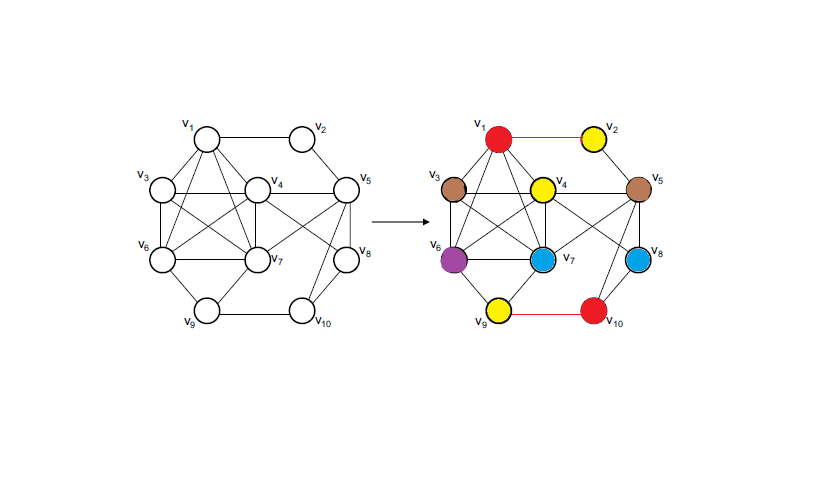
\includegraphics[width=1\columnwidth]{slike/bojanje-grafa.png}
	\caption{Bojanje grafa}
	\label{fig:bojanje-grafa}
\end{figure}

Na primjeru sa slike \ref{fig:bojanje-grafa} možemo vidjeti da je bojanje i potpuno (svim vrhovima je dodijeljena boja) i pravo (ne sadrži sudare) te time izvodljivo.


Dalje uvodimo još nekoliko pojmova.

S obzirom da više vrhova može imati istu boju, uvodi se pojam klasa boje. Ona predstavlja sve vrhove iste boje. Dakle, za određenu boju \textit{i} $\in$ {(1,..., \textit{k})}, klasa boje definirana je kao set {\textit{v} $\in$ V :\textit{ c(v)} = \textit{i}}.


Sa uvedenim pojmovima, zadatak sada možemo oblikovati na ovaj način.

Rješenje \textit{R} sastoji se od \textit{k} klasa boja  \textit{R = {$R_1$, . . . ,$R_k$}}. Pod uvjetom da je \textit{R} izvodljiv obvezno se moraju ispuniti sljedeći uvjeti:
\begin{itemize}
	\item $\bigcup\limits_{i=1}^{k} R_{i}$ = \textit{V}
	\item $S_{i}$ $\cap$ $S_{j}$ = $\emptyset$, (1 $\leq$ \textit{i} $\neq$ \textit{j} $\leq$ \textit{k})
	\item $\forall$ (u, v) $\in$ $S_{i}$, (u, v) $\notin$ E, (1 $\leq$ i $\leq$ k),
	
\end{itemize}.

Ovdje prvi i drugi uvjet zahtjevaju da svi vrhovi trebaju biti dodijeljeni točno jednoj boji u našim klasama boja. Zadnji uvjet onda kaže da niti jedan par susjednih vrhova ne smije biti u istoj klasi boja.

\newpage
\section{NP potpuni algoritam}
Bojanje grafa može biti prilično složen postupak. Krenemo li od toga da imamo \textit{n} vrhova i da ih trebamo obojati različitom bojom, mogli bi reći da uzimamo \textit{n} različitih boja i svakom vrhu možemo pridružiti jednu od tih \textit{n} boja. S obzirom da je prostor rješenja velik, broj provjera koje bi morali napraviti bio bi nepotrebno velik jer bi mogli imati $n^{n}$ različitih kombinacija rješenja, među kojima su neke od njih izvodljive. No, čak i uz limitaciju na \textit{k} boja, gdje je \textit{k} $<$  \textit{n} i dalje bi morali provjeriti velik broj kombinacija i to $k^{n}$ .\par
Iz ovog kratkog uvoda vidimo da algoritmi koji se svode na isprobavanje cijelog prostora rješenja nisu pogodni, zato što čak i na manjim instancama, izvedba bi trajala predugo. No eksponencijalni rast nije jedini razlog zbog kojeg je bojanje grafa problematično, budući da postoje  mnogi problemi koji su lagani za rješiti, također imaju veliki prostor mogućih rješenja. \par
Zahvaljujući radu Stevena Cooka koji je 1970. uveo koncepte NP kompletnosti i polinomijalne složenosti, ali je također i pokazao da  problem u kojem tražimo je li rješenje zadovoljavajuće, NP potpuni problem. Takav problem zapravo ispituje postoji li neka raspodjela vrijednosti varijablama takva da se konačno rješenje evaluira u istinito. Cook je dokazao da ne postoji algoritam koji efektivno rješava sve instance problema u kojem se traži jedno zadovoljavajuće rješenje te time označio to kao karakteristiku NP potpunog problema.\par
Dakle bitno je naglasiti da je problem u kojem se traži je li ponuđeno rješenje zadovoljavajuće, NP potpuni problem iako ne postoji algoritam koji rješava sve instance problema, ali može za ponuđeno provjeriti je li valjano. Zapravo je ovaj pronalazak doveo do zaključka da je bojanje grafa također NP potpuni problem, što ćemo sad i pokazati. Navedene zaključke možemo vidjeti ako promotrimo probleme odluke u kojima se zahtijeva da ili ne odgovor. Bojanje grafa se može postaviti kao problem odluke u kojem želimo znati možemo li graf obojati sa \textit{k} boja.\par
Problemi odluke kod kojih se izvedbeno vrijeme može izraziti polinomima, a ne kombinatornom eksplozijom, nazivaju se problemima polinomijalne složenosti.\par
Druga klasa problema odluke je NP, takozvani problemi nedeterministički polinomijalne složenosti. Problem je član NP skupa ako postoji algoritam koji za bilo koje ponuđeno rješenje može u polinomijalnoj složenosti  dati odgovor "da" ako je ponuđeno rješenje zaista rješenje problema. U našem problemu bojanja grafa  to je pitanje može li se graf obojati tako da je bojanje izvodljivo koristeći k boja. Takvo pitanje može se provjeriti u polinomijalnoj složenosti.\par
Za svaki problem koji imamo u P, možemo koristiti algoritam iz NP da provjerimo je li to rješenje problema. No i dalje se ne zna je li P = NP. To je trenutno jedan od nerješenih problema u računalnoj znanosti. Drugim riječima pitanje je može li se svaki problem čije se rješenje može brzo provjeriti zapravo i rješiti brzo.\par
No, kakogod bilo, algoritmi koji traže rješenje sa "da", trebat će pretražiti veliki prostor stanja i dalje te će rasti eksponencijalno. To implicira da ne postoji poznati polinomijalno gornje ograničen algoritam za rješavanje ovog problema.\par
Budući da se polinomijalnim transformacijama, problem bojanja grafa može svesti na problem provjere zadovoljivosti rješenja, znamo da je i bojanje grafa NP potpuni problem. 


\newpage
\section{Model ispita}
U ovom radu, raspored ispita modelirat ćemo prema sustavu sličnom kakav ima Fakultet elektrotehnike i računarstva, stoga slijedi kratki opis tog sustava.\par
S obzirom da se u ovom radu raspored izrađuje prema modelu koji je na Fakultetu elektrotehnike i računarstva poznat kao model FER3, slijedi kratki opis korištenog modela.\par
Studij na FER-u dijeli se na preddiplomski i diplomski. Kako bi student upisao diplomski, prvo mora završiti preddiplomski studij. Preddiplomski studij započinje zajedničkom prvom godinom za sve studente, a studij se organizira kroz dva programa: Elektrotehnika i informacijska tehnologija te Računarstvo. Nakon prve godine, student odabire jedan od ta dva studijska programa. Specijalizacija se unutar studijskih programa izvodi tijekom treće godine studija odabirom izbornih predmeta.\par
Upisom i polaganjem predmeta student dobiva ECTS bodove. ECTS se bodovi temelje na radnom opterećenju koje se zahtijeva od studenta, a dodjeljuju se predmetima (kolegijima) s obzirom na količinu radnog opterećenja. Tijekom svakog semestra student može minimalno upisati 24 ECTS-a, a maksimum je 37 ECTS-a nakon čega je potrebna molba za upis. Također student može upisati i predmete drugog smjera, ali uz molbu.\par
Predmeti se održavaju u dva semestra, ljetnom i zimskom. Zimski je prvi, budući da studentska godina započinje u 10. mjesecu. Tijekom zimskog semestra svaki student na Fakultetu elektrotehnike i računarstva može predmet položiti takozvanim kontinuiranim načinom u kojem student izlazi na dva ispita, međuispit i završni ispit, te pritom prikuplja bodove. Na kraju, ako je student zadovoljio sve uvjete za polaganje predmeta ne mora izlaziti na ispitni rok te je time položio predmet.\par
Ispitni je rok razdoblje u kojem student koji nije položio kontinuirano, može pokušati položiti predmet. Ispitni rok na FER-u, održava se nakon zimskog semestra, nakon ljetnog semestra te u jeseni. S obzirom da u našem modelu nećemo uzimati u obzir način polaganja predmeta preko rokova, trenutno nećemo ulaziti u dodatna objašnjavanja načina rada ispitnih rokova na FER-u.\par
U slučaju da student ne položi predmet pri prvom pokušaju, on tada ima još jedan pokušaj da položi. U suprotnom ne može nastaviti studirati na Fakuletu elektrotehnike i računarstva.\par
Preddiplomski se studij, dakle, sastoji od šest semestara, tri godine studija, a na svakoj godini, dva semestra. Na prvoj godini preddiplomskog studija svi studenti upisuju iste predmete (kolegije). Predmete preddiplomskog studija prve godine dijelimo na Obvezne predmete i Transverzalne predmete. Obvezni predmeti postoje i na drugoj i trećoj godini, te njih svaki student mora položiti. Transverzalni su predmeti, skupina predmeta od kojih student bira sebi najzanimljiviji te, po semestru student mora položiti samo jedan takav predmet. Dodatno, na trećoj se godini uvodi još jedna skupina predmeta, a to su Izborni predmeti. Među njima student bira one predmete prema području u Računarstvu u kojem se želi specijalizirati. Takvih predmeta student mora odabrati minimalno dva. Među svim tim predmetima postoje i oni koji nemaju ispite, nego je potrebno primjenom dotad stečenog znanja izraditi samostalni projekt (seminarski rad).\par 
Nakon završenog preddiplomskog studija, student ima pravo upisati Diplomski studij. No budući da se u radu osvrćemo samo na Preddiplomski studij, nećemo ulaziti u način rada Diplomskog studija.\par
U našem modelu raspored ćemo izrađivati prema opisanom modelu Fakulteta elektrotehnike i računarstva uz manja pojednostavljenja.\par
Prvo pojednostavljenje bit će to da će se model rasporeda ispita izrađivati samo za smjer Računarstvo preddiplomskog studija. Na taj način nećemo imati studente koji mogu upisati predmete smjera Elektrotehnika i informacijska tehnologija, već će svaki student u birati ponuđene predmete smjera Računarstvo. Dodatno, time nemamo niti studente koji su jedan smjer, a upisuju predmete drugog smjera.\par
Nadalje, u našem modelu, raspored ćemo izrađivati samo za zimski semestar i predmete u njemu. Time nećemo imati studenta koji na ispitnom roku može imati predmete zimskog i ljetnog semestra. Ovim načinom rada zapravo pokrivamo sve ispitne slučajeve zimskog semestra te međuispit i završni ispit ljetnog semestra. Drugim riječima, uz ovakav model, raspored ispita možemo izraditi za sve ispitne termine zimskog semestra (međuispit, završni ispit i zimski rok), a ako umjesto predmeta zimskog semestra, stavimo predmete ljetnog semestra, tada možemo izraditi raspored i za međuispit i završni ispit ljetnog semestra. Vidjet ćemo kako to možemo lako napraviti.\par
Uzet ćemo u obzir da neki od studenta druge godine upisuju predmete i prve godine i druge godine, a da neki od studenata treće godine upisuju predmete prve i druge godine. Također uzet ćemo u obzir da student treće godine neće imati upisan predmet prve godine, zbog ograničenja da student može predmet upisati dva puta.\par
Ograničenja su takva da student mora upisati minimalno 24 ECTS-a, a maksimalno 37 ECTS-a. Na taj način nećemo uzeti u obzir par rubnih slučajeva gdje studenti šalju molbe za upis više od 37 ECTS-a. \par


\newpage
\section{Problematika bojanja grafova kod izrade rasporeda}
Izrada rasporeda može se gledati kao dodjeljivanje predmeta ograničenom broju termina uz postojanje dodatnih uvjeta, među kojima će neki od njih biti opcionalni, a neki obavezni.  Jedan od uvjeta je da se ispit "A" mora održati prije ispita "B". Također uvjet može biti postavljen da se ispit "B" ne smije održati utorkom. Tu je uvjet kapaciteta, budući da fakultet ima ograničen broj mjesta u svakoj prostoriji. Naravno ne smijemo zaboraviti na glavni uvjet, a to je da se neka dva ispita ne smiju održati u isto vrijeme budući da postoji student koji piše ispit iz oba predmeta.\par
Navedene uvjete možemo podijeliti "tvrde" i "meke". Oni koji moraju biti zadovoljeni da bi se raspored smatrao "izvodljivim" zovu se "tvrdim" uvjetima. Takvi uvjeti bi bili uvjeti kapaciteta, odnosno uvjet prema kojem postoji točno određeni broj mjesta koji po svakom terminu stoji na raspolaganju. Za nas će to značiti da ćemo morati gledati koliko studenata piše ispit u određenom terminu, točnije ako postoji više predmeta koji se održavaju u istom terminu, morat ćemo gledati studente svih tih predmeta kako broj studenata ne bi bio veći od dozovljenog. Drugi takav uvjet je da se neka dva ispita ne smiju održati u isto vrijeme.\par
Uvjet koji ne moraju biti zadovoljeni, smatraju se "mekim" uvjetima. Takav je uvjet recimo da se ispit "A" ne smije održati prije ispita "B" te da ispit "B" ne smije bit u utorak.\par
Raspored će se smatrati izvodljivim ako su zadovoljeni svi "tvrdi" uvjeti.\par
U našem radu oslonit ćemo se samo na rješavanje tvrdih uvjeta, odnosno uvjeta kapaciteta i glavnog uvjeta, a to je da ne smije u istom terminu biti dva ispita takva da postoji student koji piše oba.

\chapter{Programska implementacija}
U programskoj implementaciji koristili smo programski jezi Javu. Java je odabrana zbog objektnog orjentiranog programiranja koje je potrebno za pripremu simulacije podataka, te je uz dobro odabrani algoritam dovoljno brza da može algoritam bojanja grafa korišten u radu izvesti u manje od nekoliko sekundi. Također sama prezentacija podataka bit će olakšana time zbog sučelja Swing koji koristi Java, a omogućit će prikaz rezultata bojanja grafa i prikaz rezultata izrade rasporeda.\par
U  programskoj implementaciji, kako nemamo dostupnih podataka upisa studenata na FER, morala se napraviti simulacija upisa studenata na FER. Simulaciju podataka podijelit ćemo u tri skupine te svaku ponaosob objasniti.

\section{Simulacija podataka}

\subsection*{Simulacija studenata}
Kako bi krenuli prvo smo morali simulirati studente. Kreirana su dva tekstualna dokumenta koja sadrže imena i prezimena ljudi koji se mogu pojaviti u simulaciji. Oni su kreirani tako da su posebno imena te prezimena preuzeta s Google tražilice i spremljena u dokument.
Također svaki student ima svoj JMBAG, odnosno jedinstveni matični broj akademskog građana. JMBAG je dakle jedinstven te služi za identifikaciju studenata. Također svaki student ima godinu na kojoj je upisan, upisane predmete te broj upisanih ECTS-a. Upisani predmeti dodijelit će se kasnije, ali trenutno ih je bitno napomenuti.\par
Pri stvaranju studenata prvo su izgenerirani jedinstveni JMBAG-ovi za svaku godinu, tako da počinju sa "00365", "00364" ili "00363" ovisno na kojoj godini je student.\par
Budući da smo u simulaciji pokušali stvorit što sličniji, ali pojednostavljeniji model kakav je na FER-u, uzeli smo u obzir da broj studenata na prvoj godini je 500. Na drugoj godini imamo 500 studenata od kojih 250 studenata točno druge godine, a ostalih 250 studenata što upisuju predmete prve i druge godine. Na dio sa upisom predmeta vratit ćemo se naknadno. Nadalje, broj studenata na trećoj godini 350 od čega 150 upisuje samo predmete prve godine, a ostalih 200 predmete druge i treće godine. Na dio sa upisom predmeta vratit ćemo se također naknadno.\par

\subsection*{Simulacija predmeta}
Od predmeta koje podržavamo u dostupni su svi predmeti zimskog semestra prve tri godine smjera Računarstvo na Fakultetu elektrotehnike i računarstva. Kao i ondje, predmete smo podijelili na regularne predmete, transverzalne predmete i izborne predmete. Pri tome regularni i transverzalni predmeti postoje na sve tri godine, a izborni samo na trećoj.\par
Svaki predmet ima svoje ime, broj ECTS-a koje predmet nosi te FER-ID što predstavlja identifikacijski broj predmeta na FER-u. On ujedino služi kao ID u našem modelu prema kojem se određuje jesu li neka dva predmeta ista. Također za svaki predmet određeno je ima li predmet ispit ili nema. Ovaj podatak bit će važan kasnije kod izrade rasporeda, točnije kod bojanja grafa. Ovaj dio detaljnije je opisan u dijelu \ref{sec:bojanjeGrafa}. Svaki predmet pripada određenoj skupini predmeta te se nalazi na točno određenoj godini ili više njih ukoliko je transverzalan.\par
Predmeti su ručno stvoreni u tekstualnoj datoteci. Svaka godina ima svoju tekstualnu datoteku. Također predmeti su podijeljeni u već opisane skupine, tako da nakon učitavanja podataka imamo sve predmete spremne za daljnu uporabu za simulaciju. 

\subsection*{Simulacija odabira predmeta}
U simulaciji odabira predmeta uzeli smo da svaki student upiše između 24 i 37 ECTS-a. Upisani predmeti dodijeljeni su studentu tako da u model studenta imamo kolekciju upisanih predmeta. Također svakom predmetu pridjelimo koji je student upisan na taj predmet.\par
U simulaciji dodjele studentima predmeta, pokušali smo realnije pridjeliti studentima predmete iako to nije moguće skroz točno.
Nakon što su svim studentima prve godine dodijeljeni svi predmeti prve godine, potrebno je studentima druge godine dodijeliti predmete.\par
Prvoj polovici studenata druge godine dodijeljeni su svi predmeti druge godine, s obzirom da smo uzeli da otprilike pola studenata druge godine u našem modelu je regularno upisalo drugu godinu, a druga polovica ima barem jedan predmet i prve godine. Omjer pola-pola uzet je iz iskustava dosadašnjeg stanja na FER-u, s obzirom da pokušavamo što sličije modelirati stanje FER-a. S obzirom da na drugoj godini nema još izbornih predmeta, nego samo transverzalni, postavljeno je da u obje skupine student upisuje samo jedan transverzalni predmet, a ostatak je u određenom omjeru broj predmeta prve i druge godine za onu polovicu kojoj je ostao barem jedan predmet prve godine.\par
U simulaciji predmeta treće godine imamo dodatnu skupinu predmeta, a to su izborni predmeti. Svakom studentu omogućeno je da upiše barem dva izborna predmeta, jedan transverzalni. Nadalje, ovisno kojoj skupini student pripada, dalje odabire samo regularne predmete treće godine ili odabire u određenom omjeru broj regularne predmete treće i druge godine.\par
Sada kada imamo pripremljene podatke, možemo krenuti na opis korištenih algoritama.

\newpage
\section{Algoritam bojanja grafova}
\label{sec:algoritam-bojanja}
Prije nego uvedemo algoritam bojanja grafa korišten u radu, potrebno je još uvesti model termina prema kojima smo predmete raspoređivali.

\subsection*{Termini}
U svakom terminu može se nalaziti nekoliko predmeta pod uvjetom da ta dva predmeta nemaju studenta koji piše ispit iz jednog i iz drugog predmeta. Drugim riječima, u istom terminu mogu biti samo predmeti čiji je presjek studenata koji pišu ispit iz oba predmeta, prazan skup.\par
Način određivanja broja dostupnih termina prepušten je korisniku, te ćemo u nastavku objasniti kako se on odredi. Ukoliko postoji rješenje, ti termini se dalje raspoređuju u dane, tako da u svakom danu postoji minimalni broj studenata koji će morati pisati više od jednog ispita. Ovdje više nije riječ o nemogućem scenariju.
Uzmimo da imamo studenta treće godine koji je nije položio jedan regularni predmet druge godine, te uz to upisao sve predmete treće godine. Može se dogoditi da će on u jednom danu pisati više od jednog ispita, ali u razmaku od nekoliko sati. Kako smo navodili prije "tvrde" i "meke" uvjete, ovo bi bio "meki" uvjet. Naime, trudit ćemo se da takvih studenata bude što manje, ali ne možemo garantirati da ih neće biti.

\subsection*{Priprema za bojanje grafova}
Nakon što smo studente rasporedili po predmetima, kao pripremu za bojanje grafa, treba pronaći koja dva predemeta imaju istog studenta. Problemu ćemo pristupiti tako da ne tražimo studente, zapravo mi ih već imamo te znamo koji predmeti imaju istog studenta. Dovoljno je uzeti za jednog studenta sve predmete, te budući da taj student za sve predmete koje mora pisati je ujedino i zajednički student kojeg tražimo, u nekoj strukturi, primjerice matrici, upamtimo koji su to predmeti koji imaju zajedničkog studenta. 
\newpage
\begin{lstlisting}[language = Java , frame = trBL , firstnumber = last , escapeinside={(*@}{@*)}]
graf = new int[brojPredmeta][brojPredmeta];
for (Student student : sviStudenti) {
	List<Predmet> predmetiStudenta = student.getPredmeti();
	for (Predmet p1 : predmetiStudenta) {
		for (Predmet p2 : predmetiStudenta) {
			int id1 = p1.getId();
			int id2 = p2.getId();
			if(id1==id2) continue;
			graf[id1][id2] = 1;
			graf[id2][id1] = 1;
		}
	}
}
\end{lstlisting}

Ovaj način pamćenja grafa uveli smo u ranijem poglavlju \ref{sec:teorijaGrafova} gdje smo spomenuli da vrhove pamtimo indeksima, a ukoliko postoji brid između dva vrha s indeksom n1 i indeksom n2, na to mjesto u tablici stavljamo, matica[n1][n2] = 1, te matrica[n2][n1] = 1 ako se radi o neusmjerenom grafu.

\subsection*{Backtracking algoritam}
Za bojanje grafa, točnije bojanje vrhova grafa, koristit ćemo, takozvani backtracking algoritam. Uvest ćemo prvu formalnu definiciju algoritma.\par
Backtracking je algoritamska tehnika za rješavanje problema rekurzivno tako da se pokuša rješenje postupno izgraditi, komad po komad, pri čemu se odbacuju rješenja koja ne mogu zadovoljiti zahtjeve postavljene pri rješavanju.\par
Dakle, naši predmeti bit će vrhovi, bridovi među njima postojat će ukoliko postoji student koji piše ispit iz oba predmeta, maksimalni broj dostupnih boja za bojanje grafa bit će broj termina koji nam je dostupan. Na kraju kada završimo sa bojanjem grafa, svi predmeti koji imaju istu boju, pripadat će istom terminu.\par
U radu smo uzeli da boje imaju vrijednosti od 0 do brojTermina - 1. Svakom vrhu pokušat ćemo pridjeliti najmanju dostupnu boju, ukoliko to ne bude bilo moguće zbog bilo kojeg od razloga (broj studenata u terminu je veći od dopuštenog ili dva susjedna vrha ne mogu imati istu boju), pokušat ćemo tom vrhu, točnije predmetu pridjeliti novu boju, veću od prethodne za 1, točnije novi termin, te ukoliko su uvjeti zadovoljeni, nastaviti tako bojati i ostale vrhove.\par
U ovom dijelu koda, vrijednosti boja inicijalirali smo na 0, te pozvali rekurzivnu metodu bojanjeGrafaPomocnaMetoda() s odgovarajućim parametrima. Prvi parametar je graf, odnosno matrica, kojeg smo izgradili, drugi parametar je broj dostupnih termina, treći parametar je struktura u kojoj pamtimo kojem vrhu smo pridjelili koju boju, a četvrti parametar je trenutni vrh. To je vrh s indeksom 0.
   
\begin{lstlisting}[language = Java , frame = trBL , firstnumber = last , escapeinside={(*@}{@*)}]
private boolean bojanjeGrafa(int graf[][], int brojTermina) {
	boja = new int[brojVrhova];
	for (int i = 0; i < V; i++) {
		boja[i] = 0;
	}
	if (!bojanjeGrafaPomocnaMetoda(graf, brojTermina, boja, 0)) {
		return false;
	}
	return true;
}
\end{lstlisting}

Uvjet za zaustavljanje naše rekurzivne metode je da su svi vrhovi dobili boju. Nadalje kao što smo spomenuli, pokušavamo svakom vrhu dodijeliti boju. Ukoliko uspijemo nastavljamo na novi vrh, a ako ne uspijemo, pokušavamo dodijeliti novu boju.\par
Budući da smo morali pratiti koliko studenata ima na kojem terminu, kako ne bi njihov broj postao veći od maksimalno dopuštenog po terminu, morali smo voditi računa o tome. To smo pratili na taj način da smo u svakom objektu Termina pamtili trenutno stanje predmeta koji će se tada pisati, a ukoliko ne uspijemo određenom vrhu pridjeliti trenutnu boju, taj predmet morali smo maknuti iz trenutnog termina.\par
Naime može se dogoditi da svim predmetima osim jednog uspijemo pridjeliti boju, te se tada vraćamo korak unatrag, te predzadnjem vrhu pokušavamo pridjeliti novu boju. To znači da se taj predmet neće pisati više u terminu kojem je do tada pripadao, pa moramo osloboditi mjesta zauzeta studentima tog predmeta.
\newpage
\begin{lstlisting}[language = Java , frame = trBL , firstnumber = last , escapeinside={(*@}{@*)}]
private boolean bojanjeGrafaPomocnaMetoda(int graf[][], int brojTermina, int boja[], int trenutniVrh) {
	if (trenutniVrh == brojVrhova) return true;
	for (int c = 1; c <= brojTermina; c++) {
		if (jeLiSiguran(trenutniVrh, graf, boja, c)) {
			color[trenutniVrh] = c;
			if (bojanjeGrafaPomocnaMetoda(graf, brojTermina, boja, trenutniVrh + 1)) {
				return true;
			}
			sviTermini.get(color[trenutniVrh] - 1).makniPredmet(sviPredmeti.get(trenutniVrh));
			boja[v] = 0;
		}
	}
	return false;
}
\end{lstlisting}
\medskip
\par Ova metoda služi da provjerimo možemo li određenom vrhu pridjeliti neku boju. Moramo provjeriti da njegov susjedni vrh nema tu boju te da je moguće dodati predmet u skup predmeta koji već pripadaju tom terminu.
\medskip
\begin{lstlisting}[language = Java , frame = trBL , firstnumber = last , escapeinside={(*@}{@*)}]
private boolean jeLiSiguran(int trenutniVrh, int graph[][], int boja[], int trenutnaBoja) {
	for (int i = 0; i < brojVrhova; i++) {
		if (graph[trenutniVrh][i] == 1 && trenutnaBoja == boja[i]) return false;
	}
	if (!sviTermini.get(trenutnaBoja - 1).probajDodatPredmet(sviPredmeti.get(trenutniVrh))) {
		return false;
	}
	sviTermini.get(trenutnaBoja - 1).dodajPredmet(sviPredmeti.get(trenutniVrh));
	return true;
}
\end{lstlisting}
\medskip
Ukoliko postoji rješenje možemo dalje nastaviti s raspodjelom termina po danima.
 

\subsection*{Raspodjela termina u dane}
\label{sec:raspodjelaTermina}
\par Nakon što smo dobili termine u kojima se nalaze predmeti, sada je cilj te termine rasporediti po danima kako bi dobili konačan raspored. U našoj implementaciji korištena su dva algoritma koje smo na kraju usporedili po učinkovitosti. Učinkovitost ćemo mjeriti prema broju studenata koji u jednom danu pišu više od jednog ispita.\par

\subsection*{Algoritam minimalnog presjeka}
Prvi načina koji smo koristili za raspoređivanje termina u dane je algoritam traženja trenutačnog minimalnog presjeka.
\medskip
\begin{lstlisting}[language = Java , frame = trBL , firstnumber = last , escapeinside={(*@}{@*)}]
za_svaki_termin t:
	dan<-pronadiTrenutnoOptimalniSlobodniDan(t)
	dan.dodajTermin(t)
	
\end{lstlisting}
\medskip
Ova jednostavna metoda temelji se na funkcija \textit{pronadiTrenutnoOptimalniSlobodniDan()} koja pronalazi dan u kojem bi broj studenata koji bi pisali više od jednog ispita, kada bi se dodao u njega taj termin, bio minimalan. Na kraju se doda termin u taj dan. To se ponavlja za svaki termin te se pritome ne gleda 'budućnost', odnosno što će biti dalje nakon što se doda taj termin, već samo trenutno stanje. Dakle, termini se dodaju po redu kojim su zapisani u nekom iterabilnoj listi, a za svaki se odredi dan u kojem bi presjek bio minimalan. 

\subsection*{Algoritam razdvajanja predmeta iste godine}
Drugi načina koji smo koristili za raspoređivanje termina u dane je algoritam razdvajanja predmeta iste godine.\par
Pretpostavili smo da će problem predstavljati ako se u istom danu nađu termini u kojima se nalaze predmeti prve godine te termini u kojima se nalaze predmeti druge godine. Također ukoliko se termin u kojem postoji predmet treće godine nađe u istom danu kao predmet druge godine. Razlog ovome je što postoje studenti koji su iz razloga što nisu položili sve predmete, morali upisati predmete koji su im ostali te uz to regularne predmete koje bi upisali na godini do koje su došli. Važno je napomenuti da takvi ispiti neće biti u istom terminu jer smo to bojanjem grafa onemogućili, no i dalje je moguće da kada imamo sve termine, da se takvi opisani nađu u istom danu te da to predstavlja potencijalni problem kod studenata. Nadalje, pretpostavit ćemo da svaki student piše samo jedan transverzalni predmet.\par
Također je važno reći da su ovo već "meki" uvjeti kod slaganja rasporeda te da njih nije potrebno zadovoljiti, ali pokušat ćemo što većem broju studentu naći što bolje rješenje.
Iz navedenih pretpostavki možemo dati pseudokod algoritma korištenog za raspoređivanje termina po danima.
Iz opisanog možemo dati pseudokod algoritma.\par
\medskip
\begin{lstlisting}[language = Java , frame = trBL , firstnumber = last , escapeinside={(*@}{@*)}]
transverzalni<-terminiSamoTransverzalniPredmeti()
dodajuUMinimalnomBrojuPotrebnihDana(transverzalni)

prvaG<-terminiPostojiPredmetPrvaGodinaNeDodan()
probajDodatOdvojeno(prvaG)

drugaG<-terminiPostojiPredmetDrugaGodinaNeDodan()
probajDodatOdvojeno(drugaG)

listaTrecaGodina <- preostaliTermini()
dodajSMinimalnimPresjekom(listaTrecaGodina)	
\end{lstlisting}
\medskip
\par
Prvo se dodaju svi transverzalni predmeti u što manjem broju dana, točnije da budu grupirani (ukoliko zbog broja dostupnih termina ne stanu u isti dan). Nakon toga se traže termini s predmetima prve godine koji nisu dodani i pokušava se dodat svaki u zaseban dan, a ako nije moguće, dodaje ih se tamo gdje bi bio minimalni broj studenata s više od jednim ispitom. Isto vrijedi i za termine u kojima postoji predmet druge godine, a nisu dodani. Za preostale predmete treće godine, traži se ponovno dan u kojem bi bio minimalni broj studenata s više od jednim ispitom te ga se dodaje u taj dan. Tu se opet gleda trenutno najbolje rješenje, a ne gleda se budućnost.

\newpage
\section{Aplikacija}
\subsection*{Sučelje aplikacije}
\par Pokretanjem aplikacije dobije se korisničko sučelje prikazano na slici \ref{fig:korisnicko-sucelje}.\par 
Postoje tri kartice. Prva kartica predstavlja ispis rasporeda termina po danima s predmetima, brojem termina po danu i brojem studenata koji imaju više od jednog ispita po danu. Druga kartica prikazuje graf prije nego što je obojan, uz prikazivanje svih vrhova i bridova samo za jedan vrh, budući da bi ih bilo previše, odnosno ne bi se ništa moglo vidjeti. Treća kartica prikazuje obojani graf, također samo s bridovima samo iz jednog vrha.\par
Sučelje također nudi odabir broja dana dostupnih za slaganje rasporeda, broja termina po danu te odabir načina rada. Način rada odnosi se na algoritam raspoređivanja termina po danima. Važno je napomenuti da u kojem god načinu rada pokrenuli aplikaciju, obojani graf bit će isti s obzirom da se koristi isti algoritam, prethodno opisan u poglavlju \ref{sec:algoritam-bojanja}.
\begin{figure}[h]
	\centering
	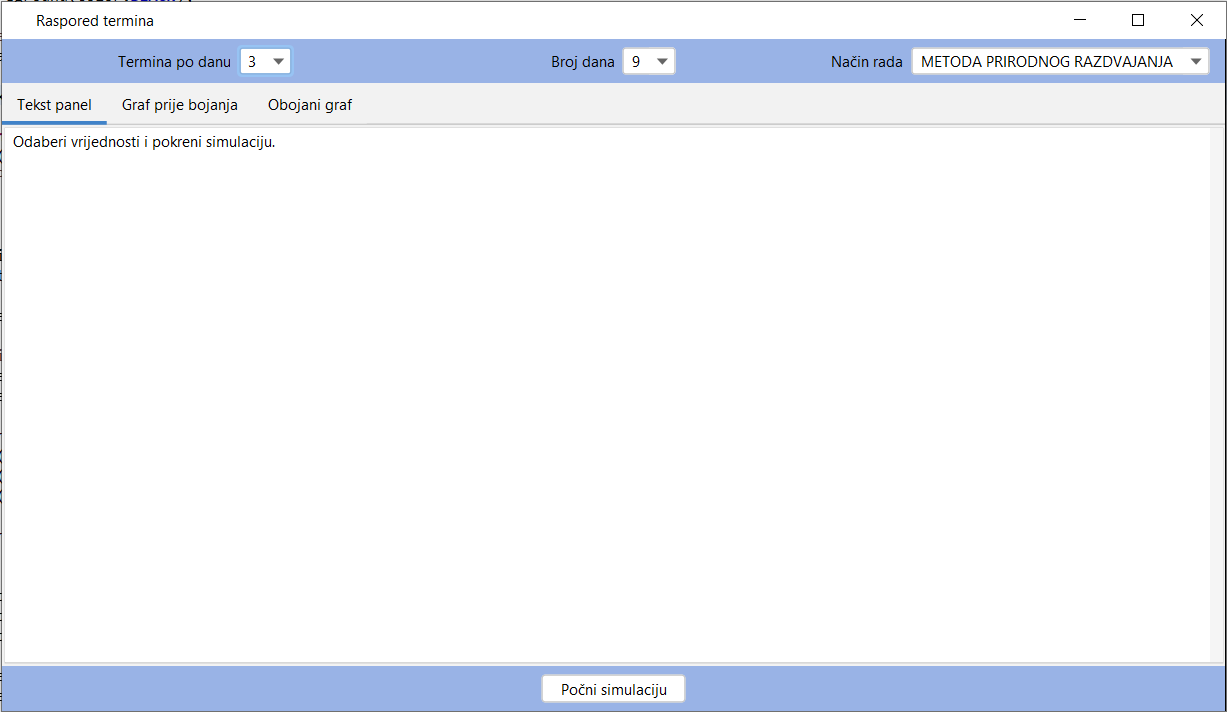
\includegraphics[width=0.9\columnwidth]{slike/aplikacija.png}
	\caption{Korisničko sučelje}
	\label{fig:korisnicko-sucelje}
\end{figure}

\subsection*{Pokretanje simulacije}
Nakon što smo odabrali broj dana dostupnih za slaganje rasporeda, te broj termina i način rada, simulacija se može pokrenuti pritiskom na tipku `Počni simulaciju`.\\

\newpage
\section{Rezultati}
Prikazat ćemo rezultate simulacije za postavljen broj dana na 9, broj termina po danu na 3 te usporediti rezultate dobivene pri istim početnim uvjetima za oba načina rada. Isti početni uvjeti odnose se na dio simulacije studenata koji su upisali predmete. Drugim riječima, prije nego se počne sa simulacijom, studentima se dodijele predmeti. Nakon toga, na temelju tih postavki, pokreću se oba algoritma.\\

\subsection{Rezultati bojanja vrhova grafa}
Prije toga potrebno je algoritmom bojanja grafa pronaći koji predmeti smiju ići u jedan termin, na temelju svih ograničenja prethodno definiranih. Ograničenja su se odnosila na kapacitete dvorana te činjenicu da predmeti ne mogu biti u istom terminu ako postoji barem jedan student koji piše oba predmeta.\par
Pokretanjem simulacije prikazat ćemo graf koji dobijemo prije nego se izvrši bojanje grafa, odnosno prikazat će se čvorovi (koji predstavljaju predmete) i bridovi između njih koji ako postoji zajednički student. Radi jednostavnosti prikaza, odnosno bolje razumljivosti, prikazat će se bridovi iz samo jednog vrha. Također prikazat ćemo koji graf dobijemo bojanjem grafa.

Sa slike \ref{fig:neobojani-graf}, možemo vidjeti da predmet Digitalna logika ne smije biti u istom terminu sa predmetima između kojih postoji brid za trenutno pokrenutu simulaciju. To su zapravo svi predmeti prve i druge godine.

\begin{figure}[h!]
	\centering
	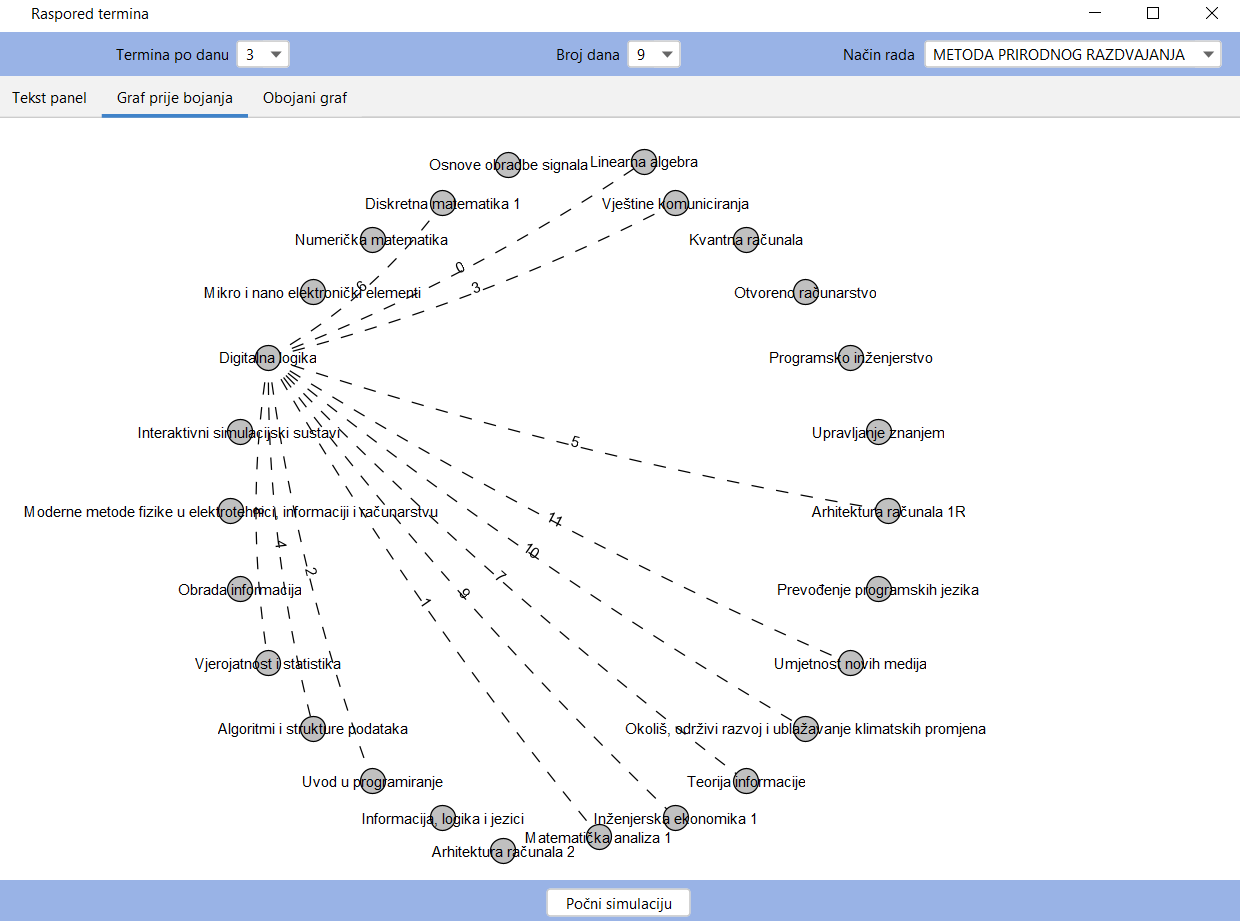
\includegraphics[width=\textwidth]{slike/neobojaniGraf.png}
	\caption{Kartica neobojani graf}
	\label{fig:neobojani-graf}
\end{figure}

Na slici \ref{fig:obojani-graf} vidimo da predmet Digitalna logika može bit, te je u istom terminu kao predmet Arhitektura računala 2, što je predmet treće godine. To ima smisla s obzirom da naša simulacije neće dopustiti niti jednom studentu treće godine da upiše predmet prve godine. Važno je dalje napomenuti da Arhitektura računala 2 nije jedini takav predmet. S njom u terminu mogu, ukoliko zadovoljavaju uvjet kapaciteta i drugi predmeti treće godine, no algoritam backtracking pronašao je prvo Arhitekturu računala 2 kao valjano rješenje.\par
Također možemo sada uočiti da svaki termin predstavlja jednu klasu boje koje imamo dostupne. Svi predmeti jednog termina pripadaju istoj klasi. Unija svih klasa su svi predmeti, a presjek bilo koja dva termina je prazan skup. Prema tome, ista klasa bili bi predmeti Digitalna logika i Arhitektura računala 2. Slično vrijedi za ostale predmete iste boje. Detaljniji ispis termina dobit ćemo u nastavku i tu možemo uočiti koji predmeti pripadaju kojoj klasi.

\begin{figure}[h!]
	\centering
	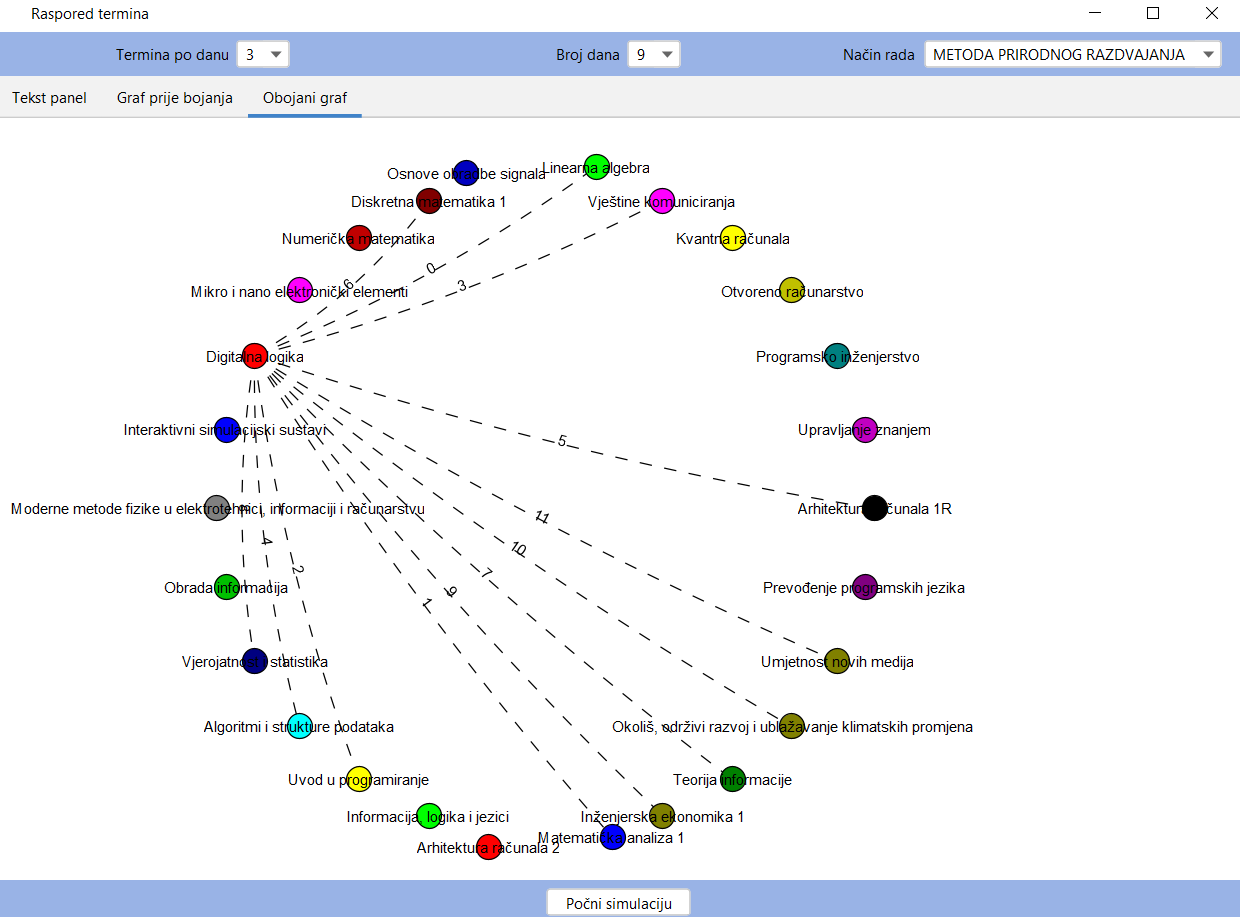
\includegraphics[width=0.9\columnwidth]{slike/obojaniGraf.png}
	\caption{Kartica obojani graf}
	\label{fig:obojani-graf}
\end{figure}
\newpage
\subsection{Rezultati metode minimalnog presjeka}
Slijede rezultati dobiveni za metodu traženja minimalnog presjeka. U ispisu možemo vidjeti koliko termina ima po danu i koliko ima studenata koji će svaki od tih dana pisati više od jednog ispita. U algoritmu za raspoređivanje termina po danima koristi se maksimalni broj dana dopuštenih za slaganje rasporeda.
\begin{figure}[h!]
	\centering
	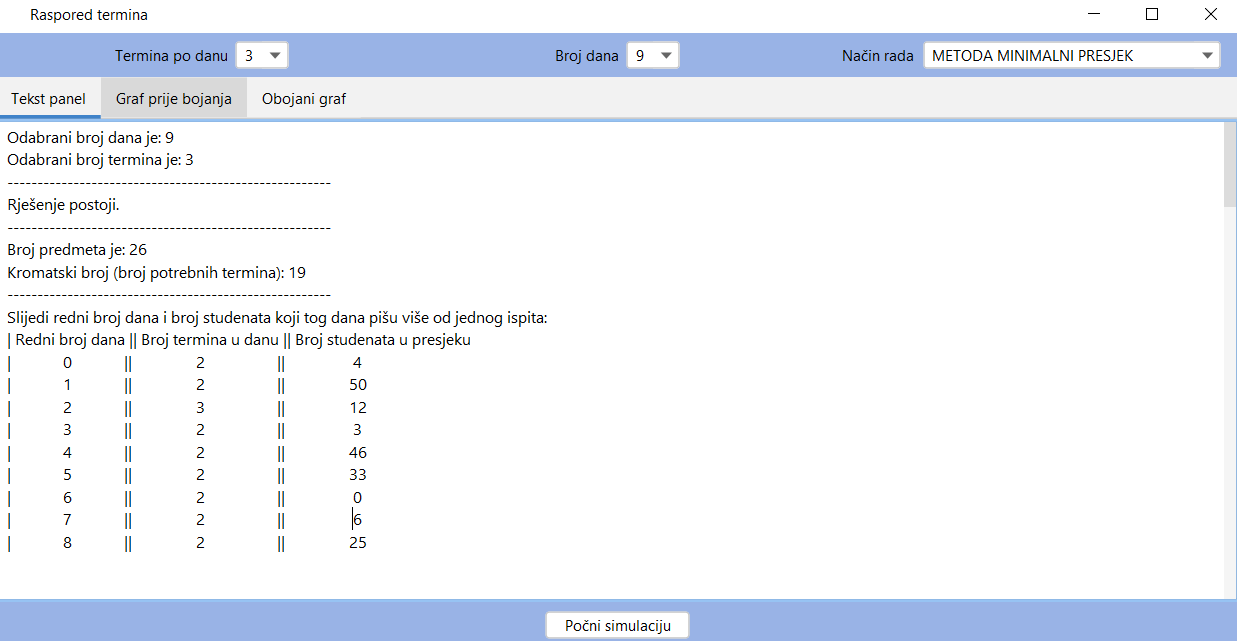
\includegraphics[width=1\columnwidth]{slike/minMetoda.png}
	\caption{Metoda minimalnog presjeka}
	\label{fig:min-metoda}
\end{figure}
Također možemo vidjeti kako su predmeti raspoređeni po terminima sa ispisom imena predmeta i godini na kojoj se taj predmet sluša. Predmeti koji su u istom terminu, na grafu prikazanom na slici \ref{fig:bojanje-grafa} obojani su istom bojom. 

\begin{figure}[h!]
	\centering
	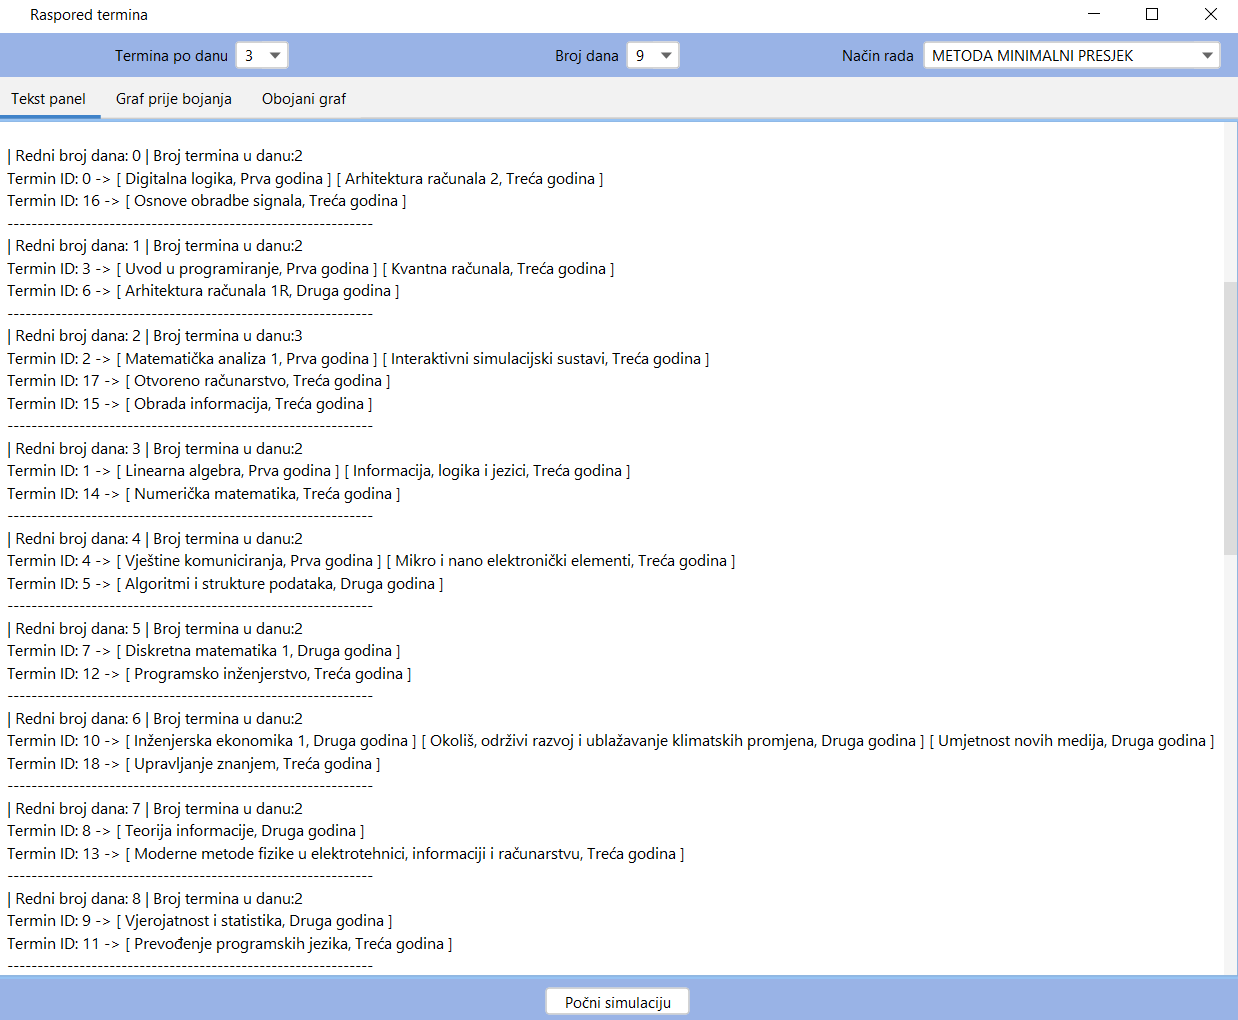
\includegraphics[width=1\columnwidth]{slike/predmetiMinMetoda.png}
	\caption{Raspored predmeta po terminima - metoda minimalnog presjeka}
	\label{fig:predmetiMinMetoda}
\end{figure}


\newpage
\subsection{Rezultati metode razdvajanja predmeta iste godine}
Slijede rezultati metode razdvajanja predmeta iste godine. Na slici \ref{fig:prirodnoRazdvajanjeRezultati} možemo vidjeti isti ispis kao i na slici \ref{fig:min-metoda}. Prikazan je broj termina po danu i broj studenata koji imaju više od jednog ispita po danu.

\begin{figure}[h!]
	\centering
	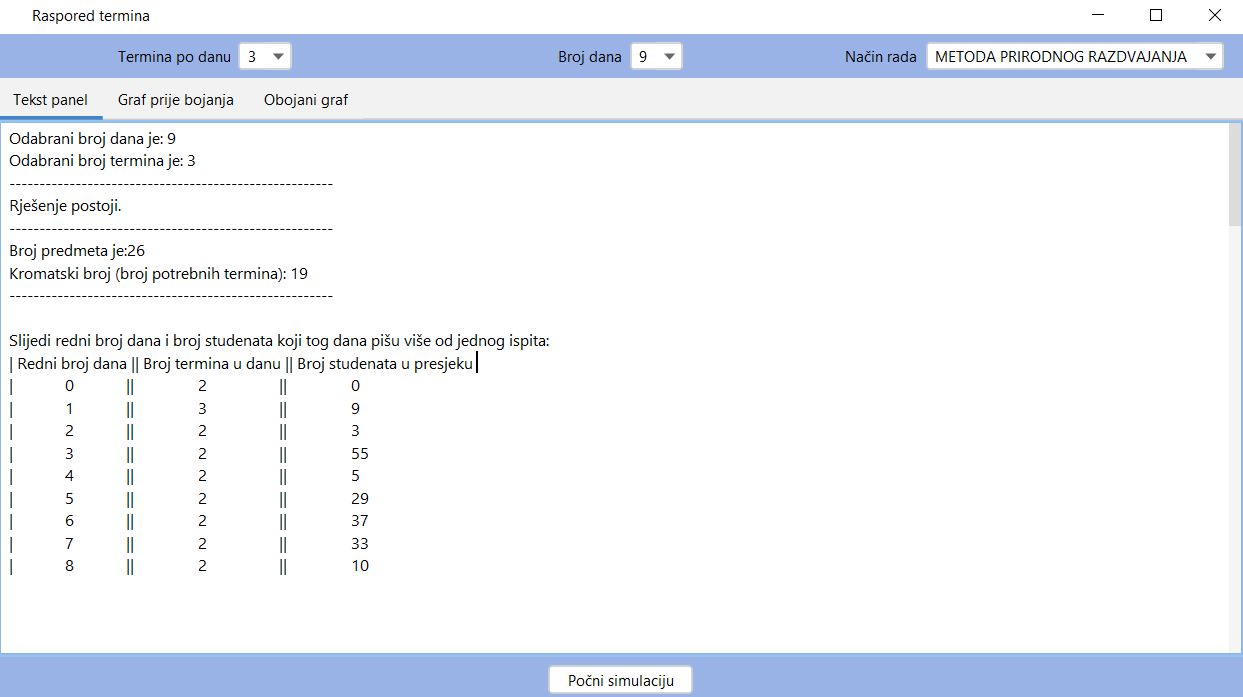
\includegraphics[width=13cm, height=8cm]{slike/prirodnoRazdvajanjeRezultati.png}
	\caption{Metoda prirodnog razdvajanja}
	\label{fig:prirodnoRazdvajanjeRezultati}
\end{figure}

Također slika \ref{fig:predmetiPrirodnoRazdvajanje} ima sličan ispis kao i \ref{fig:predmetiMinMetoda}. Na ovoj slici također vidimo iste termine, ali raspoređene na uglavnom na drugačiji način.
\begin{figure}[h!]
	\centering
	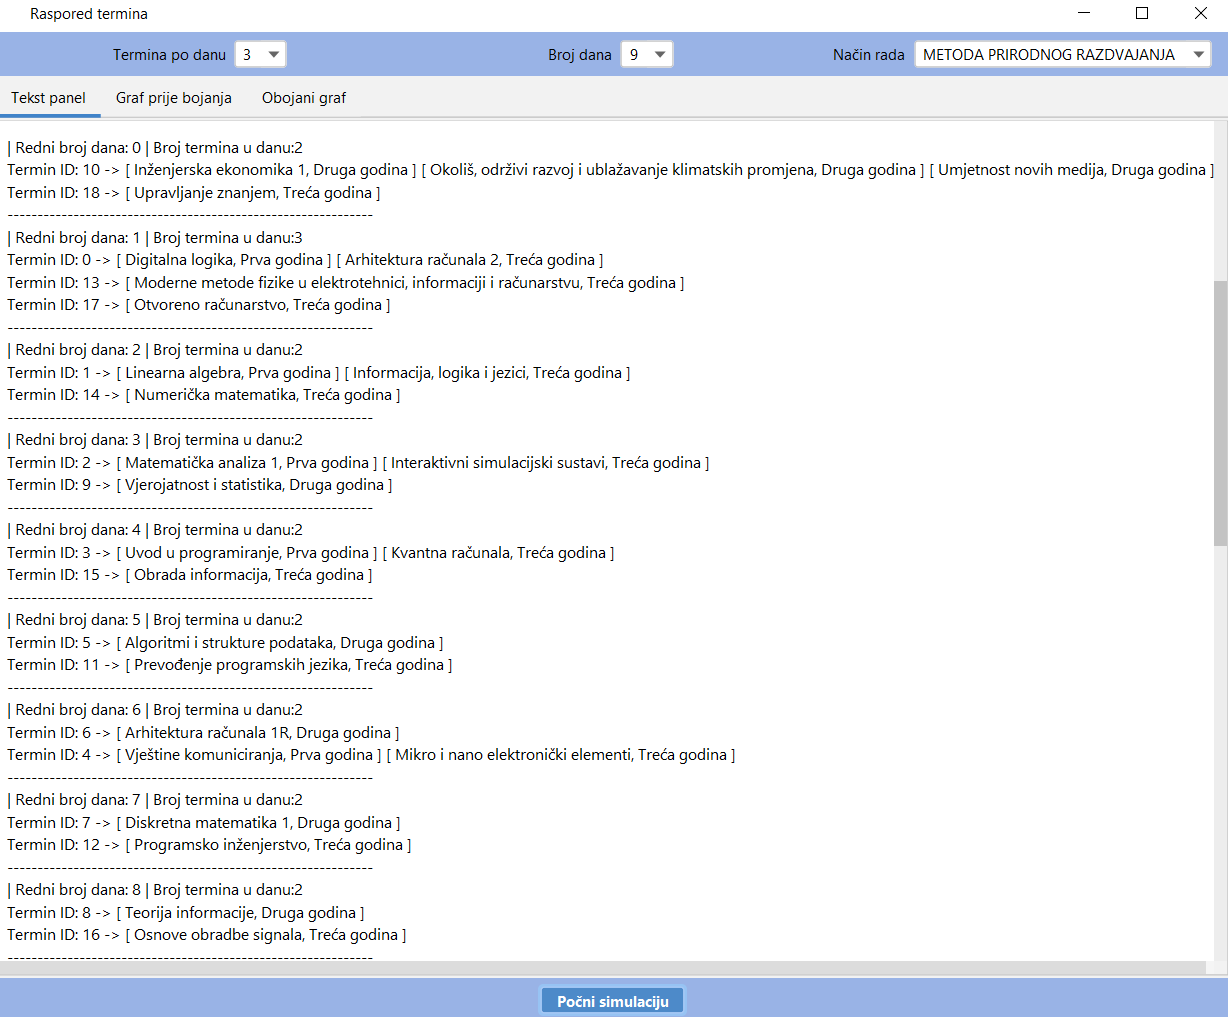
\includegraphics[width=0.9\columnwidth]{slike/predmetiPrirodnoRazdvajanje.png}
	\caption{Raspored predmeta po terminima - metoda prirodnog razdvajanja }
	\label{fig:predmetiPrirodnoRazdvajanje}
\end{figure}


\newpage~\newpage
\subsection{Usporedba rezultata i nadogradanja algoritma}
Backtracking algoritmom dobili smo raspored predmeta po terminima tako da je potreban minimalan broj dana. Zadovoljeni su uvjeti bojanja vrhova grafa.\par
Usporedbom algoritama razdvajanja predmeta sa istih godina i algoritma traženja minimalnog presjeka, uviđamo da su algoritmi otprilike jednako dobri uz malu prednost algoritma prirodnog razdvajanja budući da je i u prosjeku u više pokretanja maksimalni broj studenata koji pišu više od jednog ispita manji, ali i ukupni broj takvih studenta je manji. Razlog tome je što algoritam traženja minimalnog presjeka gleda samo trenutno stanje.\par
Algoritam se dalje može nadograditi i za smjer Elektrotehnike budući da ta dva skupa nemaju mnogo presjeka te bi samo za nekolicinu njih trebalo paziti da ne budu u istom terminu, no onda bi dalje backtracking algoritam bio prekompliciran te bi trebalo prvo tražiti razdvajanje grafa na manje podskupove i gledati što se tamo može napraviti backtracking algoritmom.\par
Kako bi se osigurala podrška za predmete ljetnog semestra, odnosno novi skup predmeta, potrebno je jedino nadograditi tekstualne datoteke koje sadrže predmete za svaku godinu ljetnog semestra.

\chapter{Zaključak}
Izrada rasporeda nije nimalo jednostavan zadatak. Mnogo je parametara u igri, od broja dostupnih dana za slaganje rasporeda, preko broja termina po danu koji ne moraju biti isti svakog dana pa sve do uvjeta koji se dodatno moraju zadovoljiti kako bi raspored bio što bolje složen. Glavni cilj ovog rada bio je složiti raspored na temelju algoritma bojanja vrhova grafa te na temelju tako dobivenih rezultata izraditi dalje raspored.\par
Kao što smo vidjeli, backtracking algoritam nudi rješenje za izradu rasporeda, odnosno raspoređivanja predmeta po terminima. Iako ne uzima u obzir cijeli prostor mogućih rješenja, nego uzima prvo koje nađe, na temelju njega mogao se izraditi pojednostavnjeni model rasporeda ispita pri čemu broj studenata koji bi pisali više od jednog ispita nije po danu u prosjeku bio veći od 20 studenata po danu kada je veći broj dostupnih dana. S obzirom da trećina studenata od njih 1350 koliko je bilo u simulaciji nije položila sve predmete, za dobiveni raspored možemo reći da je i više nego dovoljno dobar.\par
U budućnosti, osim dostupnog backtracking algoritma, skup dostupnih algoritama za bojanje grafa mogao bi se proširiti. Također, trenutne algoritme traženja trenutačnog minimalnog presjeka moglo bi se nadograditi tako da ne gledaju samo trenutno stanje, nego i buduća stanja. 
~\nocite{*}
\bibliography{literatura}


\bibliographystyle{fer}

\begin{sazetak}
Bojanje vrhova grafa je poznati NP-potpun problem iz teorije grafova. Tema rada je primjena algoritma bojanja grafova u izradi optimalnog rasporeda ispita na fakultetu tako da studenti nemaju preklapanja ispitnog termina za različite predmete. Osim same implementacije, potrebno je napraviti analizu različitih pristupa u izradi rasporeda te objasniti korištene algoritme i metode, a korisničko sučelje treba omogućiti postavljanje specifičnih parametara pri izradi rasporeda.

\kljucnerijeci{bojanje grafova, raspored ispita, matematika, algoritam, backtracking}
\end{sazetak}

% TODO: Navedite naslov na engleskom jeziku.
\engtitle{Application of Graph Coloring in Exam Scheduling Problem}
\begin{abstract}
Coloring the vertices of graphs is a well-known NP-complete problem from graph theory. The topic of the paper is the application of the graph coloring algorithm in the creation of the optimal schedule of exams at the faculty so that students do not have overlapping exam dates for different subjects. In addition to the implementation itself, it is necessary to analyze different approaches in scheduling and explain the algorithms and methods used, and the user interface should allow setting specific parameters when scheduling.

\keywords{graph coloring, shedule of exams, mathematics, algorithms, backtracking}
\end{abstract}

\end{document}
